\begin{document}

\maketitle

\section{Sissejuhatus}
\begin{frame}[fragile]
  \frametitle{Eelmine kord}
  Peamine fookus IT valitsemisel
	\begin{itemize}
		\item IT valitsemine on naljakas pool-akadeemiline distsipliin. Keeruline kunst.
		\item Äriplaan mõjutab oluliselt arhitektuurseid ja tarkvaratehnilisi otsuseid
		\item Tehniline võlg võib juhtimatuna kergesti tagumikust hammustada
	\end{itemize}
\end{frame}

\begin{frame}[fragile]
  \frametitle{Täna kavas}
		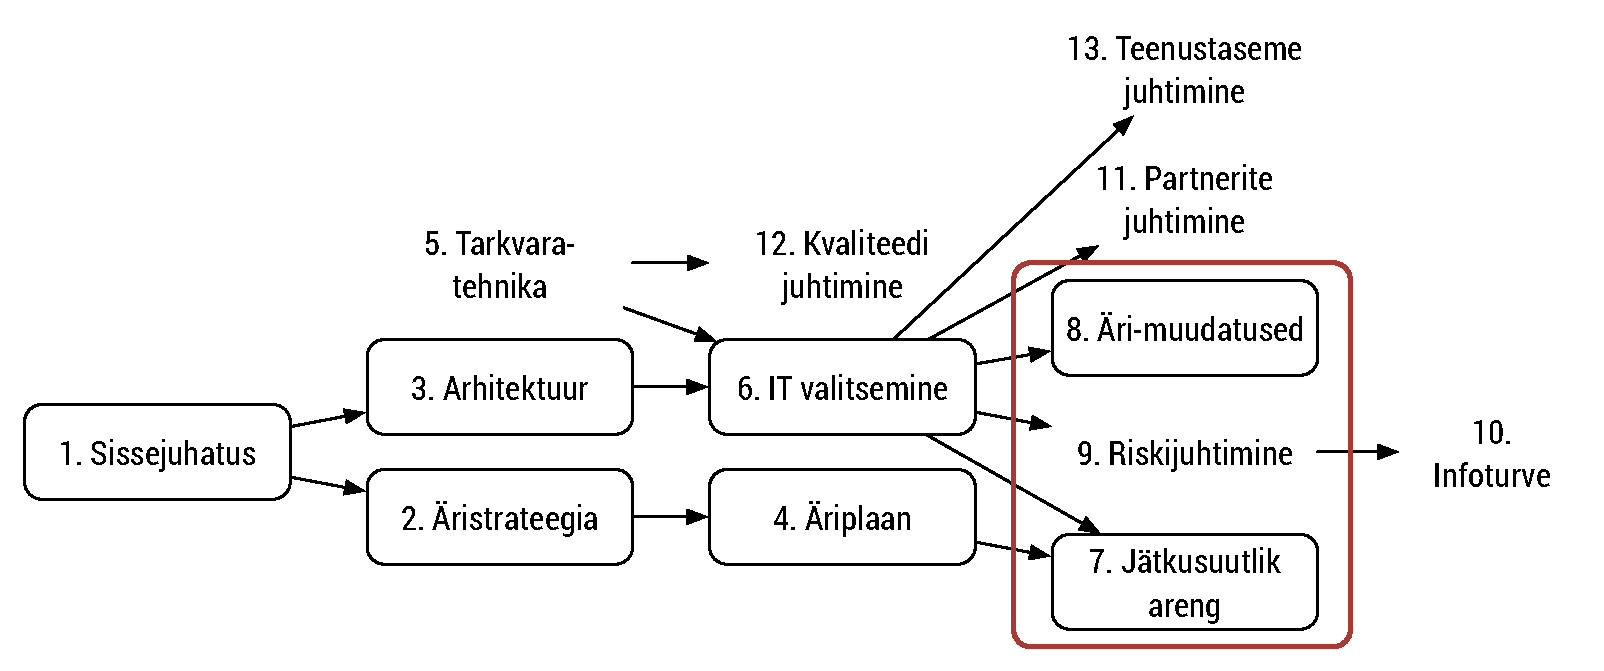
\includegraphics[width=\textwidth]{aine_struktuur_kolmas.pdf}
\end{frame}

\section{Jätkusuutlik areng}
\begin{frame}[fragile]
  \frametitle{Jätkusuutlikkusest}
  	\begin{center}
			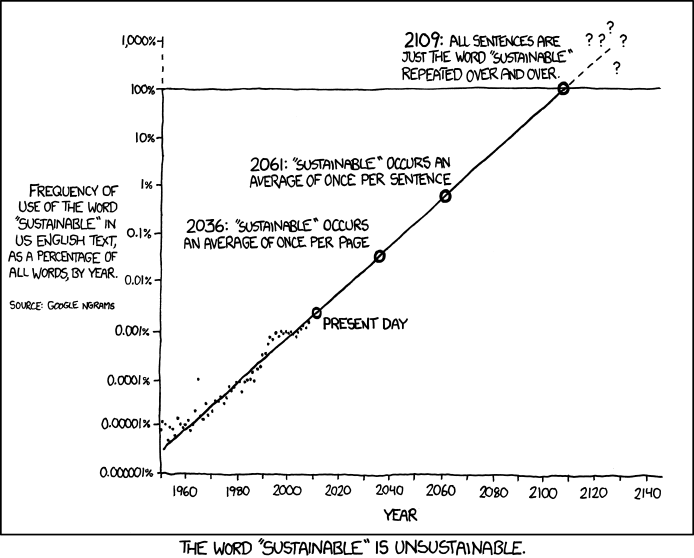
\includegraphics[width=.72\textwidth]{sustainable.png}
	\end{center}
	XKCD 1007
\end{frame}
\note{Jätkusuutlikkuse ümber on väga palju haipi ja vähe fakte. Katsuge näiteks arendada USA ajakirjanduses intelligentset vestlust kliimamuutuse ja selle põhjuste üle: saate sauna mõlemalt poolt. Katsun täna keskenduda jätkusuutlikkuse mõistele ning selle mõjule}

\begin{frame}[fragile]
  \frametitle{Jätkusuutlikkuse definitsioon}
	\begin{itemize}
		\item EKSS: arengu kohta, mis tagab inimeste elukvaliteedi paranemise kooskõlas keskkonna taluvusvõimega
		\item Wikipedia: \emph{sustainability is the endurance of systems and processes}
		\item Kas maasse augu kaevamine on jätkusuutlik tegevus?
		\item Kas 80-tunnine süsadmini töönädal on jätkusuutlik?
	\end{itemize}
\end{frame}

\begin{frame}[fragile]
  \frametitle{Jätkusuutlikkuse definitsioon}
  \begin{center}
  	\begin{quote}
		Jätkusuutlik on tegevus, mida võib mingites ajaraamides sarnaste tulemustega jätkata 
	\end{quote}
  \end{center}

	\begin{itemize}
		\item Laialt levinud definitsioonid on liiga kitsad ning ei ole otse ITle rakendatavad
		\note{Välja arvatud serveriruumide disain}
		\item Mõistes on peidus 
		\begin{itemize}
			\item ajahorisont: ka universum ei ole igavene
			\note{Keskpikas perspektiivis oleme me kõik surnud\par}
			\item ressursi mõiste: tegevuse lõppemise põhjus on ressursi lõppemine
		\end{itemize}
		
		
		\item Meie definitsiooni juured on agiilses tarkvaras \citep{sustainable}
	\end{itemize}
\end{frame}

\begin{frame}[fragile]
  \frametitle{Jätkusuutlikkus kui piirang}
 Vajadust jätkusuutlikkuse järele võib vaadelda kui kõrgemalt strateegia tasemelt seatud piirangut

	\begin{itemize}
		\item Seatakse ka muid piiranguid, neid ei tohi jätkusuutlikkusega segi ajada
		\note{Omanike otsus panna kinni tuumajaamad ja keskenduda hüdroenergiale on samaväärne otsusega mitte maksta altkäemaksu\par}
		\item Piirangud võivad tulla ka mujalt
			\begin{itemize}
				\item Riigilt
				\note{Hollandis peavad suuremahulised maasoojuspumbad näitama viie aasta lõikes null-saldot: maasse pannakse sama palju kui sealt välja võetakse\par}
				\item Kohalikult omavalitsuselt
				\item Maaomanikult
			\end{itemize}
		\item Selles kontekstis on jätkusuutlikkus nagu iga teine organisatsioonile või selle osale seatud piirang
		\note{Kui see on väline, minnakse sellest mööda kui mööda minemise kulu on väiksem, kui reeglite järgimise kulu}
	\end{itemize}
\end{frame}

\begin{frame}[fragile]
  \frametitle{Jätkusuutlikkuse ajahorisont}		
  		Jätkusuutlikkuse põhiline parameeter on ajahorisont, igal organisatsioonil on oma. Startup näeb järgmise raharingini, ülikool sajandite taha.
	  \begin{itemize}
		\item Organisatsiooni ajahorisonti mõjutavad oluliselt
			\begin{itemize}
				\item Kapitali struktuur
				\note{Kui palju on laenu- ja kui palju omanike raha. Kust omanikud raha saavad, kui pikk on laenuraha jne.\par}
				\item Omanike arusaam "väärtusest"
				\note{Iga ettevõtte ülesandeks on maksimeerida omanikele pakutavat väärtust. Börsiettevõtte ajahorisont on praktiliselt üks kvartal.\par}
				\item Keskkond
				\note{Kiiresti muutuvas keskkonnas ei ole võimalik ega mõistlik pikki sihte seada\par}
				\item Organisatsiooni strateegia
				\note{Mõnevõrra juba tulem omanike sisendist, kuid vahel mitte. On raske rääkida rohelisest ITst, kui ettevõtte strateegiaks on leida kõige odavamalt kinni makstavad ametnikud ja nende jurisdiktsioonist kuni vahele jäämiseni väärispuitu välja vedada}
			\end{itemize}		
		\item Iga juhtimistasand seab oma strateegia eelmiselt saadud piirangute alusel lisades omapoolse perspektiivi
		\note{Muude piirangute puudumisel jahutategi te oma serveriruumi hülgepoegadega, kui see juhtub kõige efektiivsem võimalus olema. Samas võib teie ajahorisont piirduda planeeritud tööajaga samas kui organisatsioon vaatab kaugemale\par} 
	\end{itemize}
\end{frame}

%Arutelu koht
\begin{frame}[fragile]
  \frametitle{Arutelu koht}
		\begin{center}
			\textbf{Miks on madal PUE oluline?}
			\note{Power Usage effectivenes}
		\end{center}
\end{frame}

\begin{frame}[fragile]
  \frametitle{Jätkusuutlikkus ja ressursid}
	Mis on see, mis võib otsa saada?

	\begin{itemize}
		\item Materiaalsed ressursid: nafta, gaas, puhas vesi aga ka inimesed
		\item Immateriaalsed ressursid
			\begin{itemize}
				\item Inimesed
				\note{Admini võimekus teha tööd, nende heasoovlikkus\par}
				\item Partnerid
				\note{Parnerite vastutulelikkus, läbirääkimissoov\par}
				\item Regulaatorid
				\note{Politseiniku soov hoiatusega piirduda\par}
				\item Ülemised juhtimistasandid
				\note{Väga oluline! Tippjuhtkond on suuteline oma soovide ignoreerimist taluma vaid piiratud hulga aega!\par}
			\end{itemize}		
		\item Oluline küsimus: \emph{360 kraadi põhimõttel ringi vaadates, milliseid ressursse sa kelleltki saad ning mida sa neile vastu annad?}
	\end{itemize}
\end{frame}

\begin{frame}[fragile]
  \frametitle{Jätkusuutlikkuse olulisusest}
	Miks üldse on oluline rääkida ja mõelda jätkusuutlikkusest?

	\begin{itemize}
		\item Ressursi lõppemine iseenesest on tavaline planeerimisülesanne ning ei ole strateegiline probleem
		\note{Me teame üsna täpselt, millal meie karjäär tühjaks saab ning saame aegsasti valmistuda uue avamiseks\par}
		\item Probleem on ülereageerimine
			\begin{itemize}
				\item Me ei pruugi teada, millal ressurss otsa saab
				\note{Seega ei saa ka planeerida. Kui kaua suudab admin 80-tunniseid nädalaid teha?\par}
				\item Me võime jätkata kulutamist ka siis, kui see tegelikult on juba otsas
				\note{Admin jätkab tööd ka pärast võimete piiri ületamist\par}
				\item Igal süsteemil on inerts, ta ei jõua hetkega reageerida
				\note{Kui admin väsib, ei ole uut kohe kuskilt võtta\par}
			\end{itemize}		
		\item Järgneb kas mõõdukas või täielik kollaps
		\note{Sõltub kasvu kiirusest ja ressursi ning kasvu reageerimisaegadest}
	\end{itemize}
\end{frame}


\begin{frame}[fragile]
  \frametitle{Jätkusuutlikkuse olulisus}
  	\begin{center}
			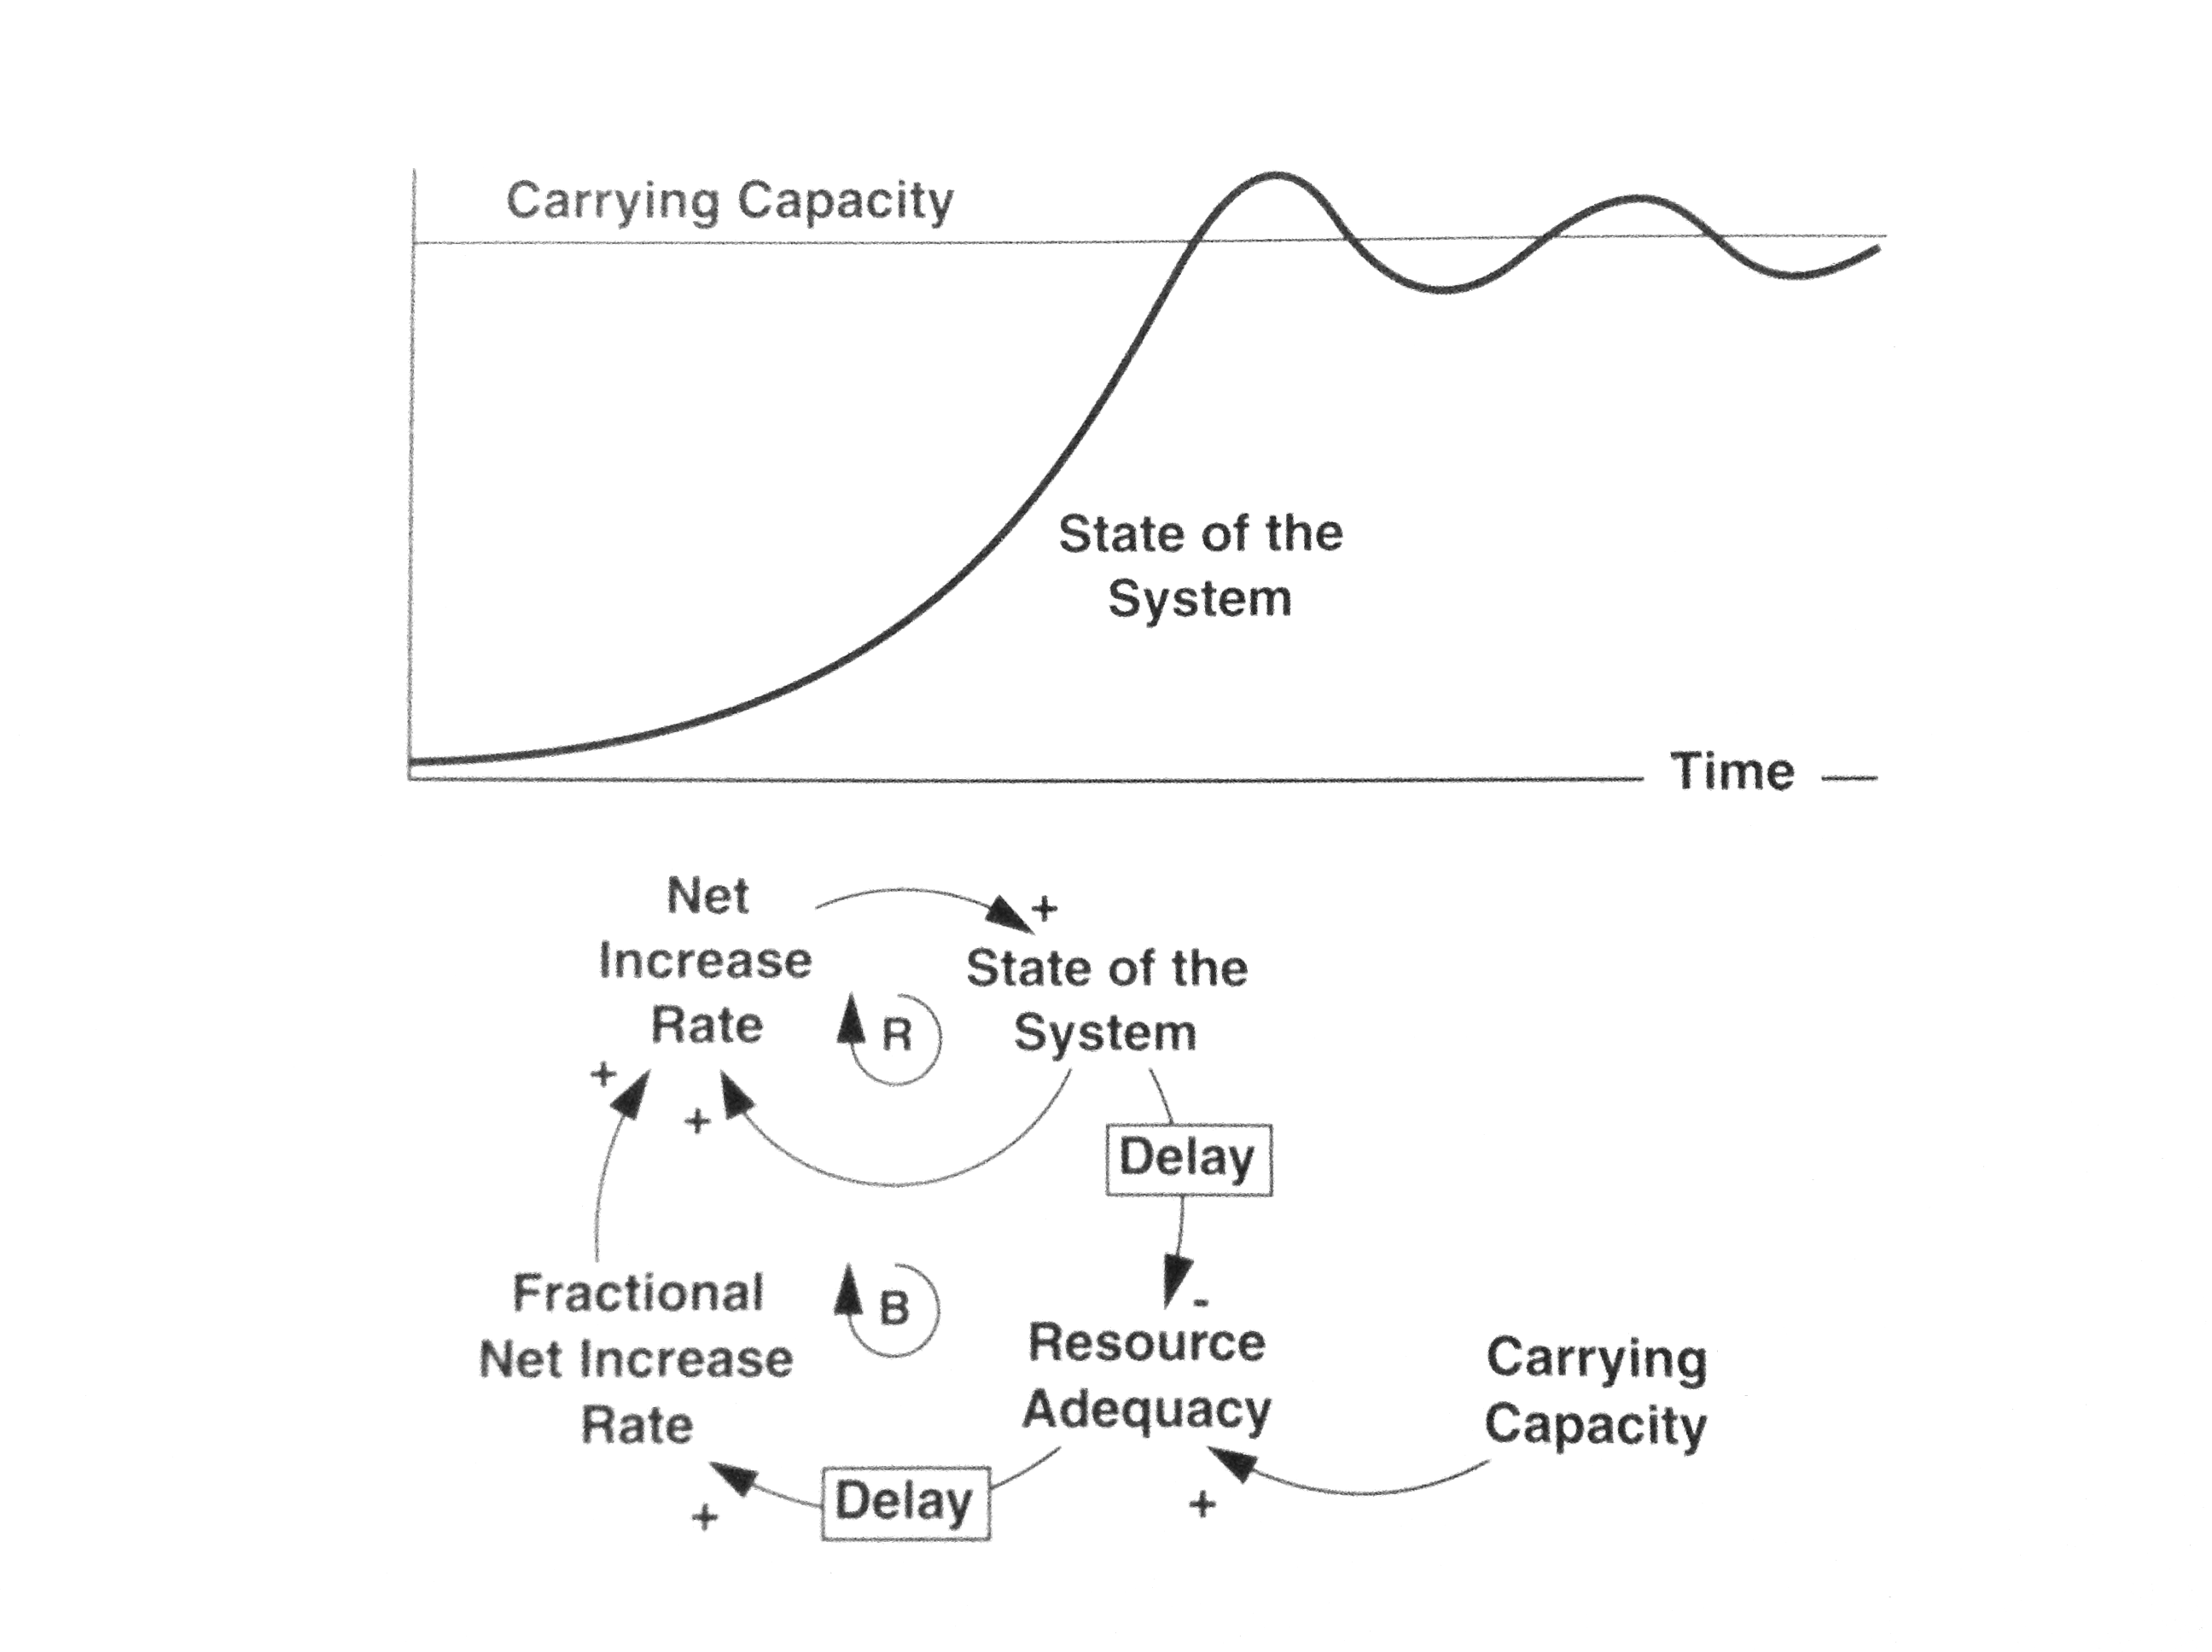
\includegraphics[width=.75\textwidth]{over.png}
	\end{center}
	\cite{sterman2000business}
\end{frame}
\note{Teised kaks stsenaariumi on S-kujuline tõus (kõige lihtsam juhtum) ning täielik kollaps}

\begin{frame}[fragile]
  \frametitle{Näide kollapsist}
	Vaatame meie süsadmini näidet. 

	\begin{enumerate}
		\item Süsadmini koormus kasvab, kuni ta teeb 80-tunniseid töönädalaid 
		\item Sellega harjutakse
		\item Admini tervis ütleb üles, ta satub haiglasse ning ei naase tööle
		\item Teil juhina on 
		\begin{itemize}
			\item Teadmuskadu admini valdusala kohta
			\note{Keegi ei dokumenteeri midagi, kui nii palju tööd teeb}
			\item Vajadus päevapealt leida \emph{kaks} uut admini
		\end{itemize}
		\item Kuni uued adminid leitakse ja käima joostakse, valitseb kaos, mis võib viia ettevõtte pankrotini
	\end{enumerate}
	Ehk, süsteemi tagasiside ei reageerinud õigeaegselt taluvuspiiri ületamisele, toimus ülereageerimine ning kas osaline või täielik kollaps. 
\end{frame}


%Arutelu koht
\begin{frame}[fragile]
  \frametitle{Arutelu koht}
		\begin{center}
			\textbf{Kuidas tuvastada jätkusuutmatust?}
		\end{center}
\end{frame}

\section{Ärimuudatused}
\begin{frame}[fragile]
  \frametitle{Miks äri muutub?}
  	\begin{center}
			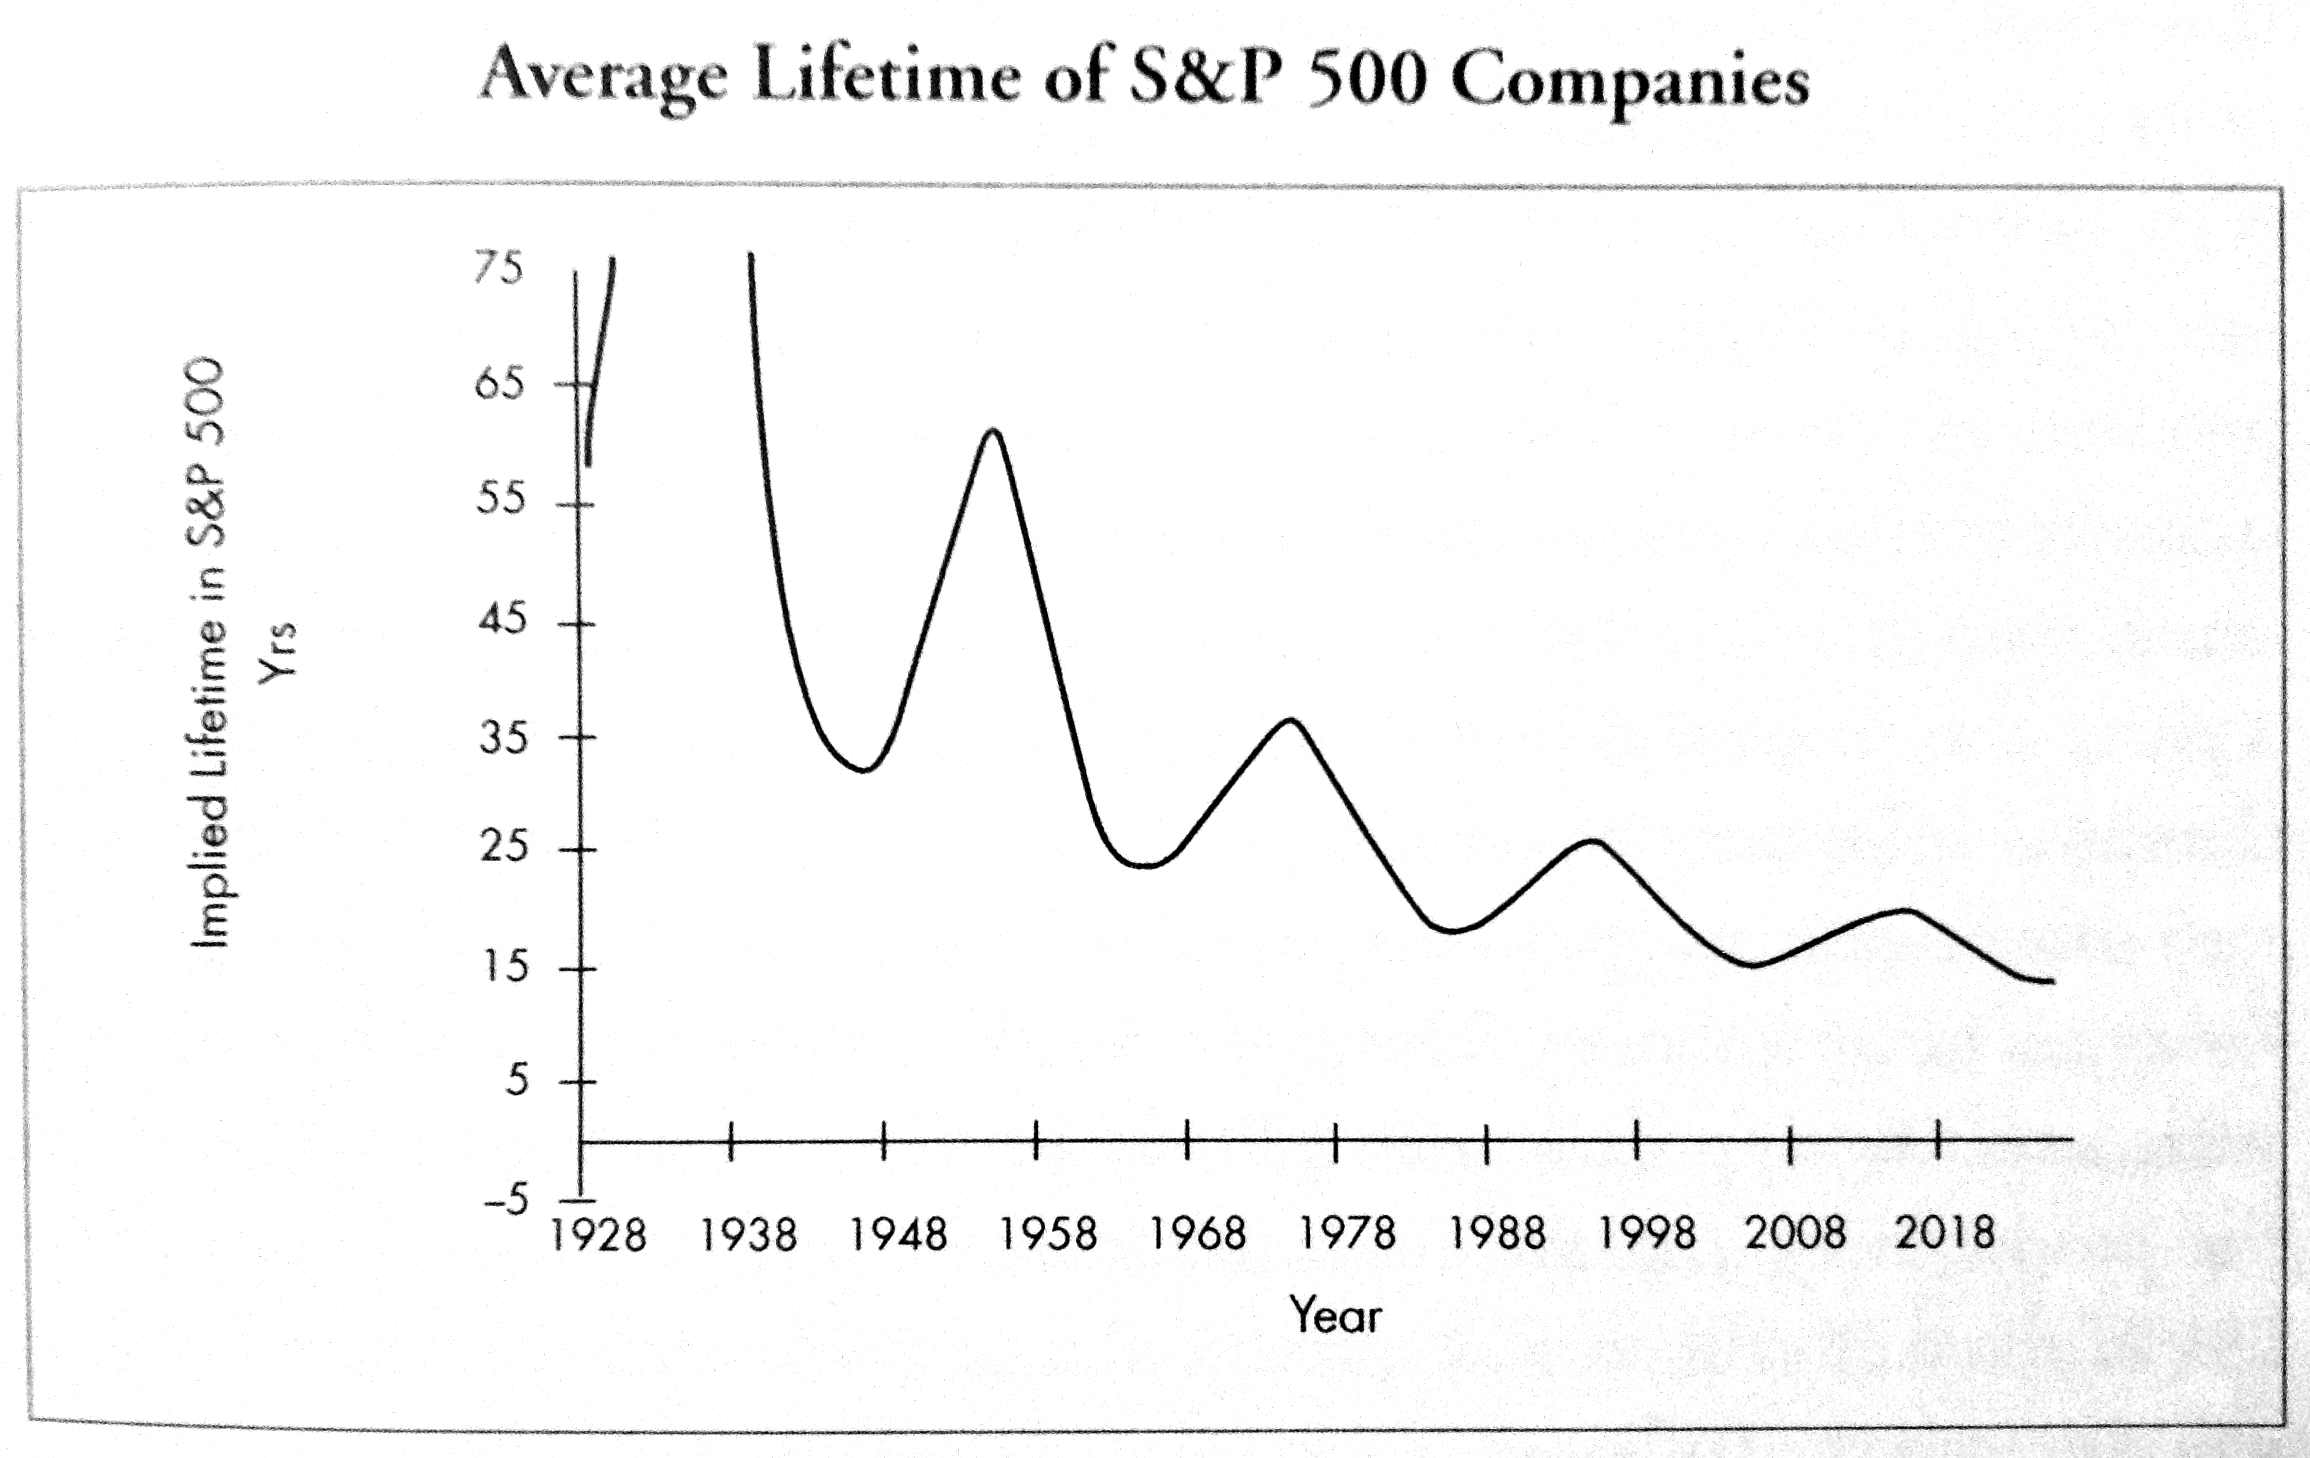
\includegraphics[width=.85\textwidth]{sp500.png}
	\end{center}
	\cite{foster2011creative}
\end{frame}

\begin{frame}[fragile]
  \frametitle{Miks äri muutub?}
  Äri muutub, sest maailm muutub. Ja muutub üha kiiremini
	\begin{itemize}
		\item 1983. aastal leidis Royal Dutch/Shell, et üks kolmandik ettevõtetest, kes olid osa F500-st seitsmekümnendatel, on kadunud \citep{senge19905th}
		\item \cite{foster2011creative} ütleb, et kestma loodud ettevõtted ei saa põhimõtteliselt edukad olla
		\item Kommunikatsioon ja globaliseerumine loovad üha mittelineaarsemat maailma
		\item Pigem peaks tekkima küsimus "miks äri juba ei muutu"?
	\end{itemize}
\end{frame}

\begin{frame}[fragile]
  \frametitle{Õppiv organisatsioon}
  \begin{center}
  	\begin{quote}
		The organizations that will truly excel in the future will be the organizations that discover how to tap people's commitment and capacity to learn at all levels in an organization
		\note{Tere Senge on väga hea. Lugege!\par}
	\end{quote}
  \end{center}
  \cite{senge19905th}
  \note{Asja mõte on, et kogu organisatsioon peab olema suuteline muutustele adekvaatselt ja paindlikult reageerima. See on spetsiifiline oskus. Dünaamilised võimekused on võtmesõna}
\end{frame}

\begin{frame}[fragile]
  \frametitle{Muutuste interferents}
  	\begin{center}
			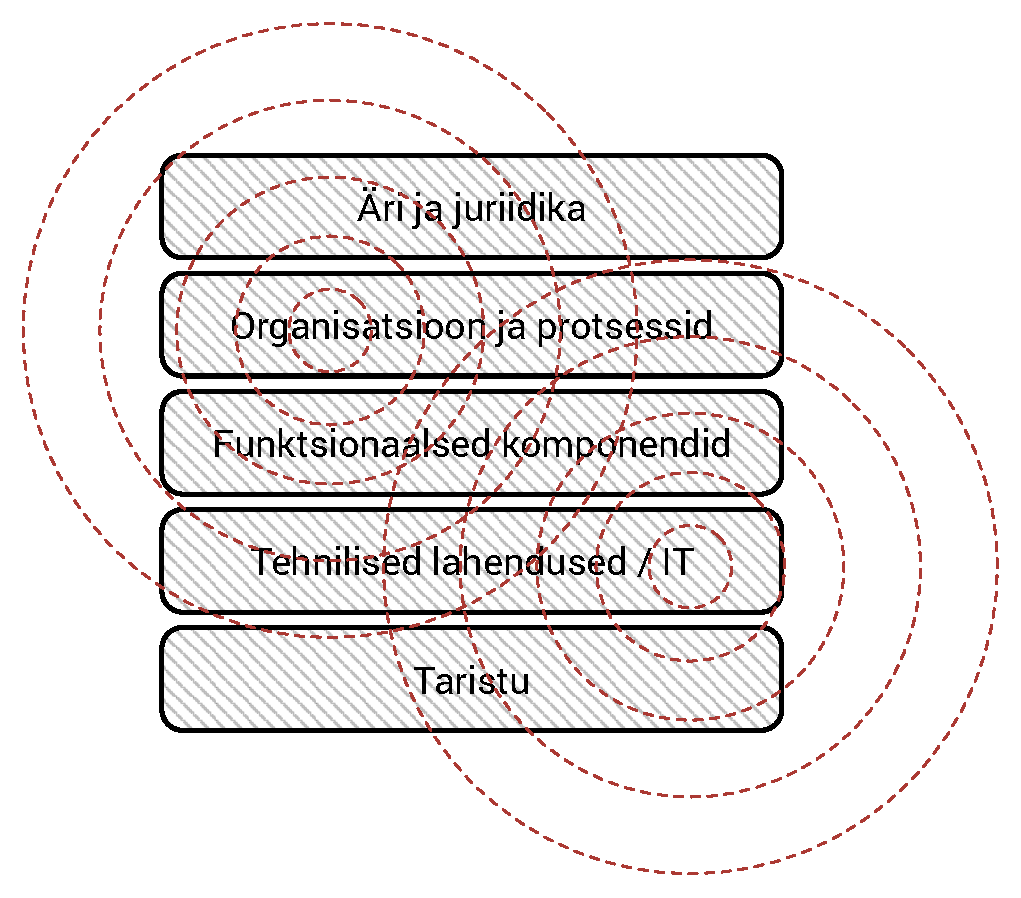
\includegraphics[width=.7\textwidth]{stack_interference.pdf}
			\note{Räägitud ka esimeses loengus. Pildi moraal: Muutused ühes kihis propageeruvad ja võivad käivitada muutusi teistes kihtides. \\ Kahe muutuse mõju kokkupuutel tekivad täiesti muudes organisatsiooni osades täiesti ettearvamatud muutused.}
	\end{center}
\end{frame}

\begin{frame}[fragile]
  \frametitle{Mida teha muutuse korral?}
  	Leia (ausad) vastused järgmistele küsimustele: 
		\begin{itemize}
			\item Mis põhjustab ärimuutuse?
			\note{Kas endogeenne või eksogeenne muutus?\par}
			\item Milles muutus seisneb?
			\note{Ehk, mis täpselt muutub. Neid kahte tuleb omavahel valideerida kuid 100\% vastavust ära oota, vt. British Steeli näide edaspidi\par}
			\item Kes kontrollib muutust?
			\note{Kes vastutab. Väga oluline küsimus. Väga hea vastus on ka vastuse puudumine\par}
			\item Millistes organisatsiooni kihtides on muutus struktuurne ja millistes mitte?
			\note{Mäletate, rääkisime arhitektuurist kui parameetrite vektorist. Arhitektuuri muutmine on kallis, parameetrite muutmine odav\par}
			\item Milline on muutuste kadents?
			\note{See on väga oluline küsimus: kas te peaksite oma süsteeme ehitama paindlikumaks või mitte. Paindlikkus on kallis, seda ei ole mõistlik niisama tekitada.\par}
		\end{itemize}

\end{frame}


%Arutelu koht
\begin{frame}[fragile]
  \frametitle{Arutelu koht}
		\begin{center}
			\textbf{Kas IT saab algatada organisatsiooni äri muutuse? \\Kui jah, siis kuidas?}
		\end{center}
\end{frame}

\begin{frame}[fragile]
  \frametitle{Keerukus}
	\begin{itemize}
		\item Keerukuse eksponentsiaalne kasv üle võimete piiri
	\end{itemize}
\end{frame}

\begin{frame}[fragile]
  \frametitle{Mis on keerukus?}
  	\begin{center}
			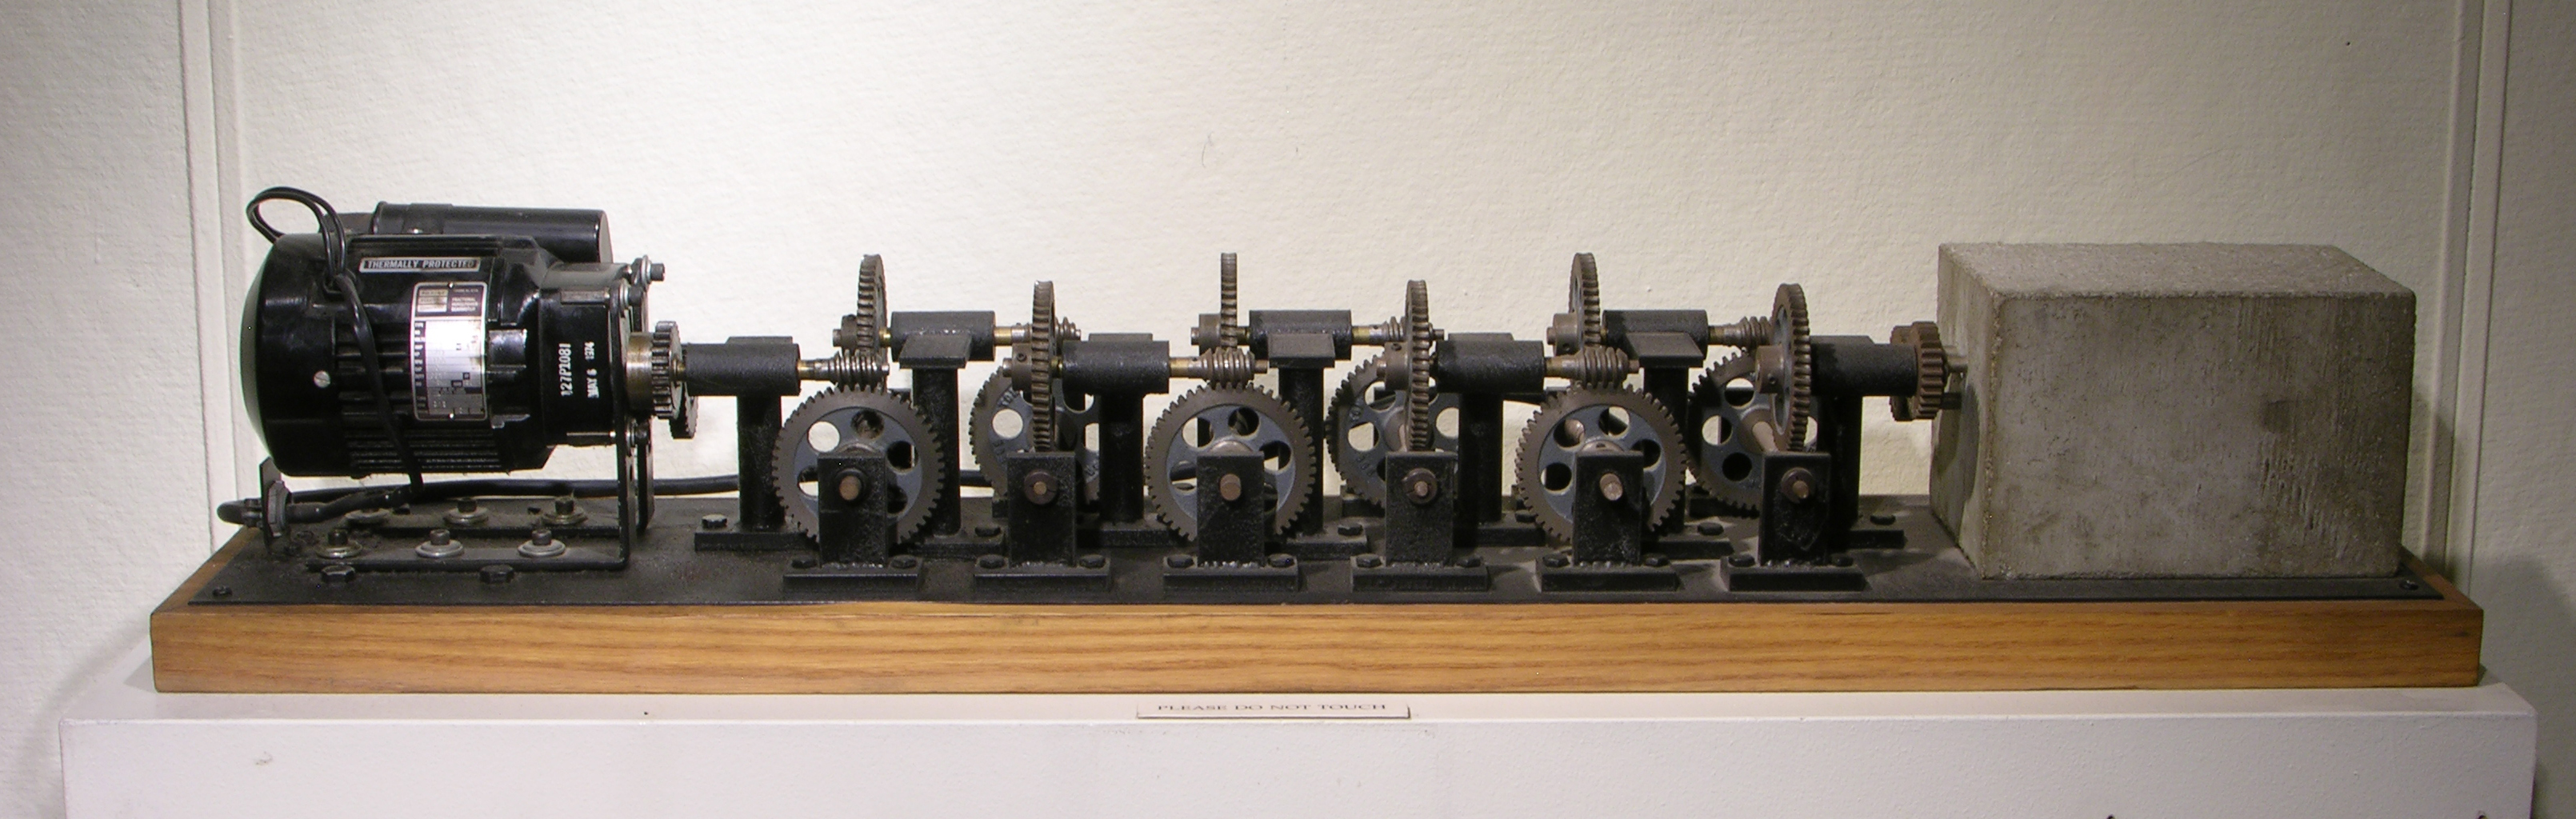
\includegraphics[width=\textwidth]{concrete.jpg}
			\note{Mootor 200 rpm, 12 ülekannet, iga ülekanne vähendab 50 korda. Viimane võll pöörleb kord kahe triljoni aasta jooksul. Kui toda võlli keerata kiirusega 1 m/s ja masin vastu peaks, pöörleks mootor 814 365 469 korda valguse kiirusest kiiremini\\}
	\end{center}
	Arthur Ganson, Machine with Concrete
	\note{Ei ole teada, millal tehtud. Arvatavasti asub Exploratoriumis SFis\\Suurepärane näide dünaamilisest keerukusest ja eksponendi rollist selles}
\end{frame}

\begin{frame}[fragile]
  \frametitle{Miks rääkida keerukusest?}
  Iga muutus äris on olemuslikult muutus keerulises sotsiotehnilises süsteemis
	\begin{itemize}
		\item IT-juht vastutab selle süsteemi tehnilise osa eest
		\note{Erinevalt "sotsio" poolest ei saa siin hakkama deklaratsioonidega, keerukust ignoreerida ei saa\par}
		\item IT-juhi roll on juba niigi keerulises süsteemis viia läbi mittetriviaalne muutus
		\item Kuna ei ole ruumi rääkida süsteemiteooriast, räägime keerukusest
		\item Arusaam keerukuse olemusest annab head mõttemudelid keerulistest situatsioonidest mõtlemiseks
	\end{itemize}
	\note{Keerukusest on oluline aru saada ning ärimuudatused tundus olevat õige koht sellest rääkimiseks}
\end{frame}

\begin{frame}[fragile]
  \frametitle{Keerukuse mõiste}
  Ühest definitsiooni ei ole. On viisid selle mõõtmiseks \citep{mitchell2009complexity}:
  \note{Meil juba olid sellised asjad: strateegia, arhitektuur... Võib olla on tegu lihtsalt keelelise abstraktsiooniga, mille taga ongi hulk eri nähtusi?}
	\begin{itemize}
		\item Keerukus kui suurus, osiste ja nendevahelise seoste hulk
		\note{Kõige levinum inseneerias. Küllalt intuitiivne.\par}
		\item Keerukus kui entroopia määr
		\note{Shannon entropy. Üllatuse määr kommunikatsioonis\par}
		\item Keerukus kui pakitavuse määr
		\note{Kui palju annab süsteemi kokku pakkida. Tehniliselt Algorithmic Information Content\par}
		\item Keerukus kui loogiline või termodünaamiline sügavus
		\note{Kui keeruline on süsteemi konstrueerida. Loogiline on matemaatliselt kena Turingi masina kaudu defineeritav konstruktsioon, praktiliselt aga kasutu. Termodünaamiline on samuti keeruline\par}
		\item Keerukus kui sisendi ja väljundi seos
		\note{Statistiline keerukus. Minimaalne kogus infot praeguse ja eelnenud sisendi kohta, mida on vaja väljundi ennustamiseks. Dünaamiline keerukus!\note}
		\item Keerukus kui fraktaaldimensioon
		\note{Matemaatika, fraktalid, liiga keeruline, et siin detaili minna. Lugege}
		\item Keerukus kui alamsüsteemide hulk
	\end{itemize}
\end{frame}

\begin{frame}[fragile]
  \frametitle{Veel keerukusest}
	Keerukust saab jagada veel eri dimensioone pidi:
	
	\begin{itemize}
		\item Dünaamiline ja staatiline keerukus
			\begin{itemize}
				\item Dünaamiliselt keerukas süsteem käitub kaootiliselt: kuitahes väike sisendi muutus võib põhjustada kuitahes suure muutuse väljundis
				\note{Liblika tiivalöök ja Bono. Meie süsteemid käituvad tänapäeval samuti\par}
				\item Staatiliselt keerukas süsteem on keerulise struktuuriga
				\note{Staatilist keerukust mõõdab enamus eeltoodud meetrikaid.\par}
			\end{itemize} 
		\item Tehniline ja äriline keerukus
			\begin{itemize}
				\item Tehniliselt keerulise süsteemi mõistmiseks peab omama sügavaid teadmisi arvutiteadusest  
				\note{Selline on näiteks Skype p2p võrk\par}
				\item Äriliselt keerulise süsteemi mõistmiseks peab omama sügavaid teadmisi ärist
				\note{Selline on näiteks Skype veebipood.\par}
			\end{itemize} 
		\item Keerulisus vs. keerukus
			\begin{itemize}
				\item Keerulisus (ingl. \emph{complicatedness}) on süsteemi omadus näida keeruline
				\item Keerukus (ingl. \emph{complexity}) on süsteemi keerukuse määr
				\note{Väga ohtlikud on madala keerulisusega keerukad süsteemid. How hard can it be?\par}
			\end{itemize} 
	\end{itemize}
\end{frame}

\begin{frame}[fragile]
	\frametitle{Võtmeküsimus:}
	\vfill
	\begin{center}
		Milline on teie süsteemi keerukus eri mõõdikute järgi?  
		\note{Sellest sõltub, kuidas ja mil viisil saab hinnata ärimuutuse mõju teie poolt juhitavale süsteemile ning teie võimekust reageerida}
	\end{center}
	\vfill
\end{frame}



\begin{frame}[fragile]
  \frametitle{Mis on keerukus?}
  	\begin{center}
			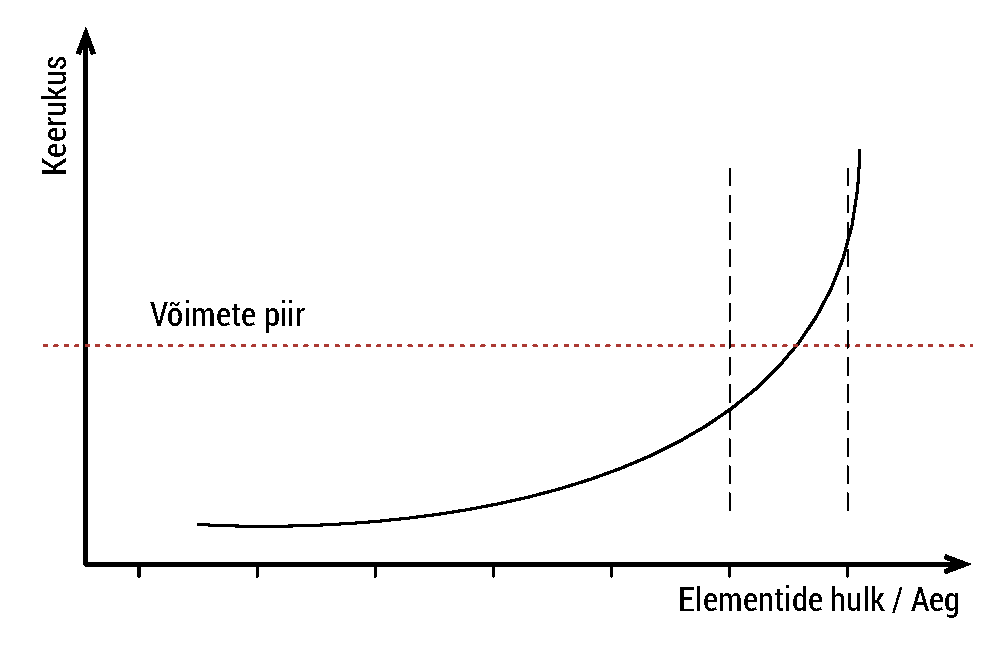
\includegraphics[width=.7\textwidth]{keerukus.pdf}
	\end{center}
	Keerukusel on komme kasvada mittelineaarselt. Suhteliselt väike samm horisontaalteljel võib organisatsiooni paigutada suhteliselt kaugele teisele poole oma võimete piire. 
	\note{Tegu on abstraktsiooniga! Elementide hulk ajas tavaliselt kasvab. Ja piir ei ole teada. Ja keerukuse dimensioone on palju.}
\end{frame}

\begin{frame}[fragile]
	\frametitle{Võtmeküsimus:}
	\vfill
	\begin{center}
		Kui kaugele minu võimete piirist \\mind käesoleva muutusega surutakse?
		\note{Ma võin toime tulla muutusega aga kas ma suudan muutuse järel tekkinud süsteemi ka üleval pidada ning järgmistele muutustele viia?}
	\end{center}
	\vfill
\end{frame}


\begin{frame}[fragile]
  \frametitle{Keerukuse juhtimine}
  	Keerukuse juhtimine on vastava taseme arhitekti töö. 
	\note{Meie puhul IT juhi oma \par}
	On järgmised põhimõttelised strateegiad
	\begin{description}
	\item[Google mudel:] Joone tõusu vähendamine
	\note{G suudab lisada teenuse teenuse ja serveripargi serveripargi järel ilma, et ta oma kompetentsist üle kasvaks}
	\item[Morgani mudel:] Peatumine horisontaalteljel
	\note{Morgan keeldub kasvamast, sest muidu satuks ohtu nende operatsioonimudel. Samal põhjusel ei võta pangad teatud piirist kallimaid projekte ette}
	\item[Skype mudel:] Võimete piiri tõstmine
	\note{Skype tagas, et suudab palgata kõige paremad saadaolevad insenerid ja lasta neil rahus toimetada viies sellega üles oma võimekuse. Ühel hetkel sai piiravaks juhtkonna võimekus}
\end{description}
\end{frame}


%Arutelu koht
\begin{frame}[fragile]
  \frametitle{Arutelu koht}
		\begin{center}
			\textbf{Mida teha, kui ees olev muutus viib organisatsiooni teisele poole oma võimete piiri?}
		\end{center}
\end{frame}

\begin{frame}[fragile]
  \frametitle{British Steel}
	\begin{itemize}
		\item 1975. aastal pidi British Steel Corporation otsustama, kas ja kui mitu uudse tehnoloogiaga tehast Korfi korporatsioonilt osta 
		\item Granada Television filmis kogu protsessi
		\item Filmis jookseb korduvalt läbi fraas "kas üks või kaks tehast"
		\item Strateegiline analüüs näitas, et tehast ei pruugi üldse vaja olla
		\item Lõppotsus: osta kaks uue tehnoloogiaga tehast
		\note{Põhjused mitmetahulised. Muu hulgas öeldakse, et aeti segi kaks eri otsust: kas uus või vana tehnoloogia ning kas osta või mitte osta. Oma rolli mängis ka ettevõttesisene poliitika.\\}
		\item Neist üks pandi püsti kuid konserveeriti kohe. Teist ei pandud kunagi püsti ning müüdi alles mõned aastad tagasi
	\end{itemize}
	\begin{center}
		\textbf{Moraal:} ära kunagi eelda, et otsustusprotsess on ratsionaalne
	\end{center}
\end{frame}

\begin{frame}[fragile]
	\frametitle{Pank}
	\vfill
	\begin{center}
		Näide ühe nimetuks jääva finantskorporatsiooni\\ ärimuutuse mõjust ITle
		\note{Kuigi jutt tugineb avalikele allikatele, vääriti mõistmise välimiseks juhtumit lahti ei kirjuta}
	\end{center}
	\vfill
\end{frame}

\begin{frame}[fragile]
  \frametitle{Kaduv disain}
  Kuidas ja miks 90ndatel veebi toel tekkinud Digitaalse Muutuse Agendid on nüüdseks kadunud \citep{design}. 
	\begin{itemize}
		\item Kogu veebidisaini äri sai võimalikuks vaid tänu veebile
		\item Tekkis täiesti uus ärivaldkond
		\item Disain muutus kriitiliseks edufaktoriks
		\note{Google Ventures design for equity idee\\}
		\item Suurkorporatsioonid tajusid strateegilist riski ja tõid disaini majja
		\note{IBMil ~1000 disainerit palgal, Barclays suurim disainimaja Londonis jne.\\}
		\item Tulemus: põhimõtteliselt on muutunud viis, kes ja kuidas tänapäeval kasutajakogemust disainib
		\begin{itemize}
			\item Muutunud on kogu \emph{toolchain}
			\note{suurtel on jõudu mõjutada JSi ja brauserite arengut, kus on Dreamweaveri ja FrontPage analoogid?}
			\item UXi disain on integraalne osa tarkvara arendamise protsessist
			\note{Kuigi meie tarkvaratehnika osas sellest palju ei rääkinud? How come?}
			\item On tekkinud reaalne \emph{design divide}
		\end{itemize}		
	\end{itemize}
\end{frame}

%Arutelu koht
\begin{frame}[fragile]
  \frametitle{Arutelu koht}
		\begin{center}
			\textbf{Kas strateegilised otsused peaksid olema ratsionaalsed?}
		\end{center}
\end{frame}

\section{Riskijuhtimine}
\begin{frame}[fragile]
  \frametitle{Riskijuhtimine}
	\begin{itemize}
		\item System safety mõiste
		\item Põgus ülevaade eelduste muutusest
	\end{itemize}
\end{frame}

\begin{frame}[fragile]
  \frametitle{Riskijuhtimine}
	
	\begin{itemize}
		\item Enamasti ei saa rääkida IT riskide juhtimisest eraldi organisatsiooni riskide juhtimisest
		\item Süsteemide keerukuse kasv muudab põhimõtteliselt riskide juhtimise olemust
	\end{itemize}

	\begin{center}
		\emph{Ei ole sisulist vahet, kas elektrijaam plahvatab kellegi rumaluse, küberründe, disainivea või komponendi kulumise tõttu}
		\note{Inimesed saavad surma ja suur kahju tekib igal juhul}
	\end{center}
\end{frame}

\begin{frame}[fragile]
  \frametitle{Muutused riskijuhtimises}
	Järgnev kehtib üha enam kõigi riskitüüpide puhul
	\begin{itemize}
		\item BCP\footnote{\emph{Business Continuity Plan}} keerukus/hind kasvab eksponendina süsteemi keerukusest
		\item BCP efektiivsus kahaneb eksponendina süsteemi keerukusest
		\item Üksikute riskisündmuste asemel peame rääkima pidevast, kasvavast ja kuju muutvast survest
		\item Riskifaktoreid ei saa enam suruda aktsepteeritavale tasemele
	\end{itemize}
\end{frame}

\iffalse
% Need slaidid tõstetud märkmetesse, aega ei ole
\begin{frame}[fragile]
  \frametitle{BCP keerukus}
	BCP keerukus/hind kasvab eksponendina süsteemi keerukusest
	\begin{itemize}
		\item Facebookil ei ole kuskil teist andmekeskust igaks juhuks jõude seismas. See oleks liiga kallis
		\item Väliste partnerite puhul ei ole alati võimalik alternatiivi leida
		\item Äriprotsesside toimimisele ei ole vahel enam mitte-elektroonilist alternatiivi
	\end{itemize}
\end{frame}

\begin{frame}[fragile]
  \frametitle{BCP efektiivsus}
	BCP efektiivsus kahaneb eksponendina süsteemi keerukusest
	\begin{itemize}
		\item Kuidas taastub pilveteenusepakkuja täielikust andmekaost?
		\item Keerulist süsteemi ei pruugi õnnestuda ka mitte ajuti taastada, kui palju ka ei kulutaks
		\note{Kui Skype p2p võrk päriselt maha kukub, seda sisuliselt ei olnud võimalik taastada}
		\item Äriplaanid, kliendiandmed, ideed, dokumentatsioon on üha enam immateriaalne ja seega kergesti teisaldatav
	\end{itemize}
\end{frame}

\begin{frame}[fragile]
  \frametitle{Voog sündmuste asemel}
	Üksikute riskisündmuste asemel peame rääkima pidevast, kasvavast ja kuju muutvast survest
	\begin{itemize}
		\item Ka kuritegevuses on edukas see, kes suudab oma ärimudeli võimalikult efektiivselt võimalikult suureks skaleerida
		\item Keerulises süsteemis on väga palju elemente ja nende interaktsioone, mõne katki mineku tõenäosus on suur
		\note{Suures tehases läheb kogu aeg midagi katki}
		\item Inimese kognitiivset võimet ületavate süsteemide puhul kasvab kiiresti operaatori vigade tõenäosus
		\note{Mistõttu ma olen suhteliselt ettevaatlik Eesti Vabariigi infosüsteemi torkimisega}
	\end{itemize}
\end{frame}

\begin{frame}[fragile]
  \frametitle{Riskifaktorid}
	Riskifaktoreid ei saa enam suruda aktsepteeritavale tasemele
	\begin{itemize}
		\item Riik suudab tagada, et tänaval ei jookse nagaaniga vehkiv jõuk, internetis ei ole see võimalik
		\item Süsteemi kõik elemendid ei ole kontrolli all
		\note{Vt. esimese kontakti slaidid Yosemite intsidendist}
		\item Kuna info liigub, kerkib kiiresti esile uusi (Google: \emph{"ATM gas attacks"})
		\item Turvalist ega vigadeta tarkvara ei ole reaalne toota
		\note{Heartbleed istus aastaid laialt kasutatud open source tarkvarateegis kõigi silmade all}
	\end{itemize}
\end{frame}

\fi
% Siit edasi on jälle OK

\begin{frame}[fragile]
	\frametitle{Kuidas läheneda?}
	\vfill
	\begin{center}
		Keeruliste probleemide puhul küsi alati: \\kellel on sama probleem akuutsemalt ja kauem?  
		\note{ABS leiutati kõigepealt lennukite pidama saamiseks. Autoinsenerid said lahenduse sealt}
	\end{center}
	\vfill
\end{frame}

\begin{frame}[fragile]
  \frametitle{Süsteemiohutusest}
	Keerukate süsteemide ohutuse eest hoolitsevatel inimestel on asjakohane teooria ja praktika olemas.
	\begin{itemize}
		\item Kuidas tagada USA tuumalaevastiku ohutus?
		\note{5400 reaktori-aastat intsidentideta tööd}
		\item Keemiatööstus, lennukid, laevad 
		\item Juured ICMB ja Apollo programmides eelmise sajandi keskel
	\end{itemize}
\end{frame}

\begin{frame}[fragile]
  \frametitle{Süsteemiohutuse definitsioon}
	\begin{center}
		\begin{quote}
			This system safety standard practice is a key element of Systems Engineering (SE) that provides a standard, generic method for the identification, classification, and mitigation of hazards.
		\end{quote}
	\end{center}
			MIL-STD-882
	
\end{frame}

\begin{frame}[fragile]
  \frametitle{Süsteemiohutusest}
	Levinuimad põhjuslikkuse mudelid eeldavad, et õnnetusi põhjustavad komponentide rikked ning et neid rikkeid vältides või neiks valmistudes võib õnnetusi vältida. Kuigi see eeldus on tõsi lihtsate elektromehaaniliste süsteemide puhul, pole see enam nii tänaste keeruliste sotsiotehniliste süsteemide korral \cite{leveson2011engineering}.
	\begin{itemize}
		\item Rida varasemalt toiminud eeldusi enam ei kehti
		\item Põhjused on nii süsteemide keerukuse tõusus kui ka maailma järjest keerulisemaks muutumises
		\note{Tuletage meelde juttu süsteemi piiridest}
		\item Võtmetähtsusega on sotsiotehniliste süsteemide vaatlemine terviklike, tagasisidestatud mittelineaarsete süsteemidena
	\end{itemize}
\end{frame}


%Arutelu koht
\begin{frame}[fragile]
  \frametitle{Arutelu koht}
		\begin{center}
			\textbf{Kui tõsine probleem on riskijuhtimise paradigma muutus \\tegelikus elus?}
		\end{center}
\end{frame}


\section{Viited}

\begin{frame}[t,allowframebreaks,]
  	\bibliographystyle{plainnat}
	\bibliography{it_strateegia} 

\end{frame}

%\plain{Küsimusi?}
\begin{frame}[plain]
	\begin{center}Küsimusi?\end{center}
\end{frame}


\end{document}